%\chapter{\normalsize{BACKGROUND OF SATELLITE REMOTE SENSING}}
\chapter{\normalsize{RESULTS}}
\paragraph{}
This chapter deals about the outcome of our analysis and how to share the results with the community.
%\section{Technique 5: Processing satellite data using GIS Software}
\section{Extract chart command line tools.}
\subsection{Visualise temperature chart.}
The script below show how to extract temperature chart from GRASS GISS using command line.
\newline
The same code work for others meteorological parameters (Wind, Surface Pressure, Relative Humidity), we just need to change
few parameters in the script.
\begin{lstlisting}[language=Bash]
# Visualize data
#Set date and time on 31 January 2021 at 03:00 UTC
dt="20210131.0300"
#Set date and time on 31 January 2021 at 03:00 UTC
#dt="20210131.1500"
# Open a monitor
d.mon wx0
#set the coordinate grid
d.grid 3
# Display a raster map
d.rast GLDAS_NOAH025_3H_A${dt}_Tair_final
# Display a vector map
d.vect map=cmr type=boundary
#Add text
#d.text text="31 JAN 2021 0300Z" color=black bgcolor=white size=3
d.text text="31 JAN 2021 1500Z" color=black bgcolor=white size=3
# Add raster legend
# Add raster legend
d.legend -t -s -b raster=GLDAS_NOAH025_3H_A${dt}_Tair_final title=TEMPERATURE title_fontsize=20 font=sans fontsize=18
# Add North arrow
d.northarrow style=1b text_color=black
#clear the monitor
#d.erase -f
# press enter
\end{lstlisting}
\begin{figure}[H]
\begin{center}
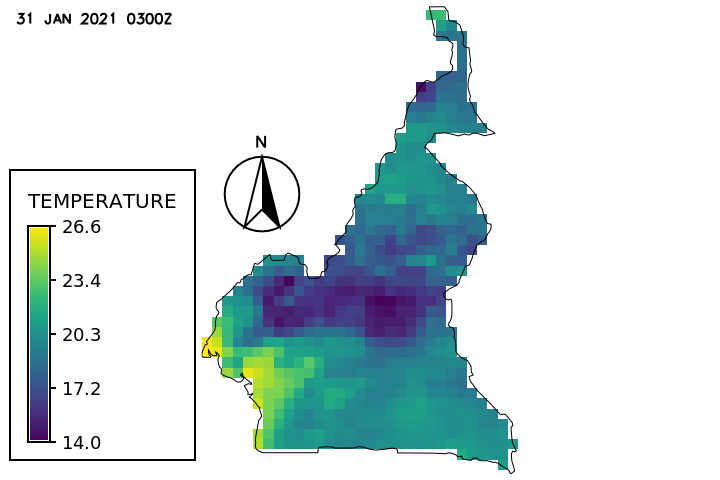
\includegraphics[scale=0.6]{tp03.png} %\cite{umhe}
\end{center}

\caption{Temperature at 03:00 UTC}
\label{Temperature at 03:00 UTC}%\cite{ABIA}
\end{figure}
\begin{figure}[H]
\begin{center}
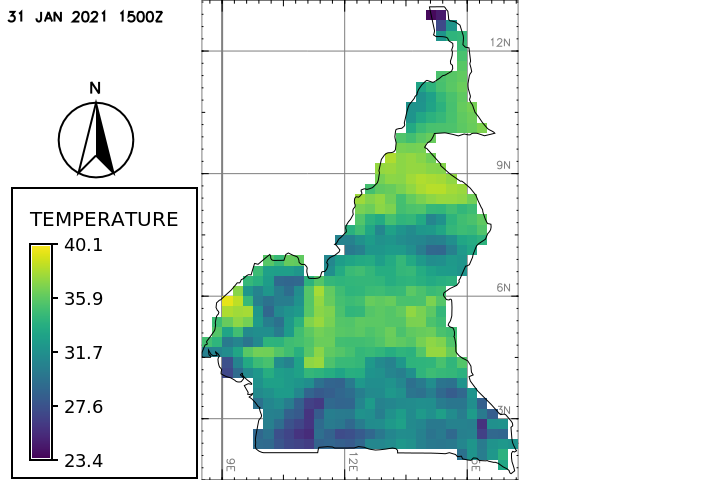
\includegraphics[scale=0.6]{tp15a.png} %\cite{umhe}
\end{center}
\caption{Temperature at 15:00 UTC}
\label{Temperature at 15:00 UTC}%\cite{ABIA}
\end{figure}

\subsection{Visualise Relative Humidity Chart}
\begin{figure}[H]
\begin{center}
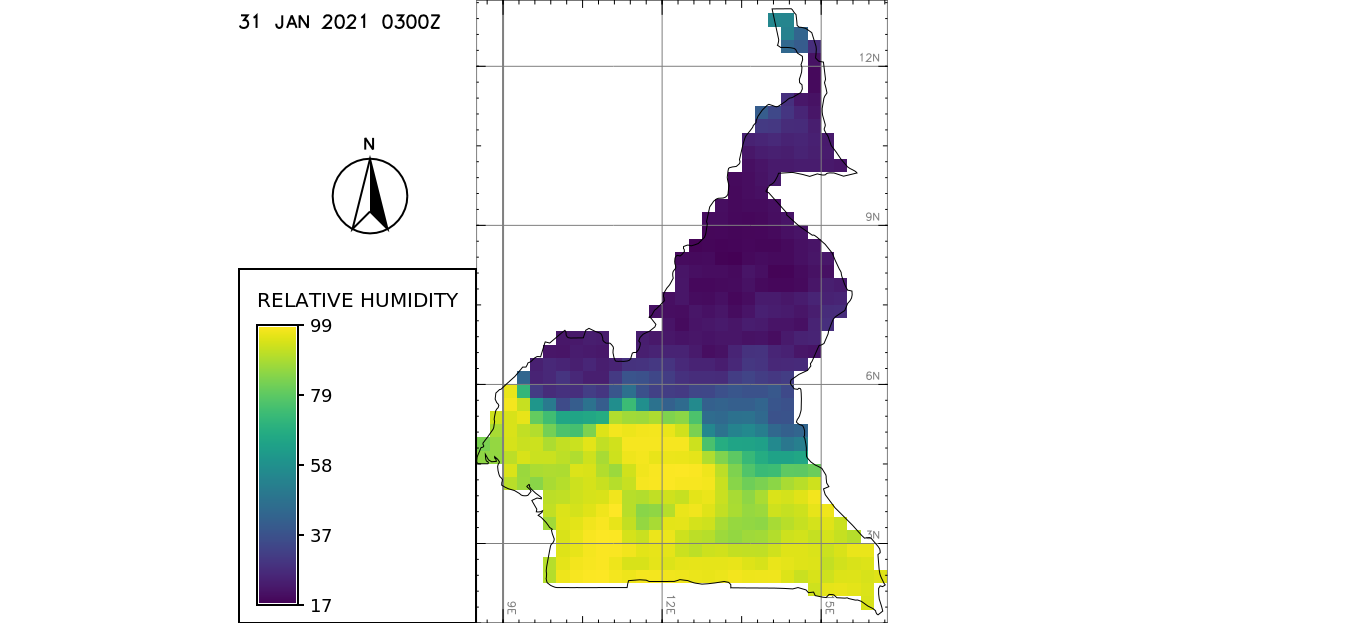
\includegraphics[scale=0.4]{rh3a.png} %\cite{umhe}
\end{center}
\caption{Relative Humidity at 03:00 UTC}
\label{Relative Humidity at 03:00 UTC}%\cite{ABIA}
\end{figure}

\begin{figure}[H]
\begin{center}
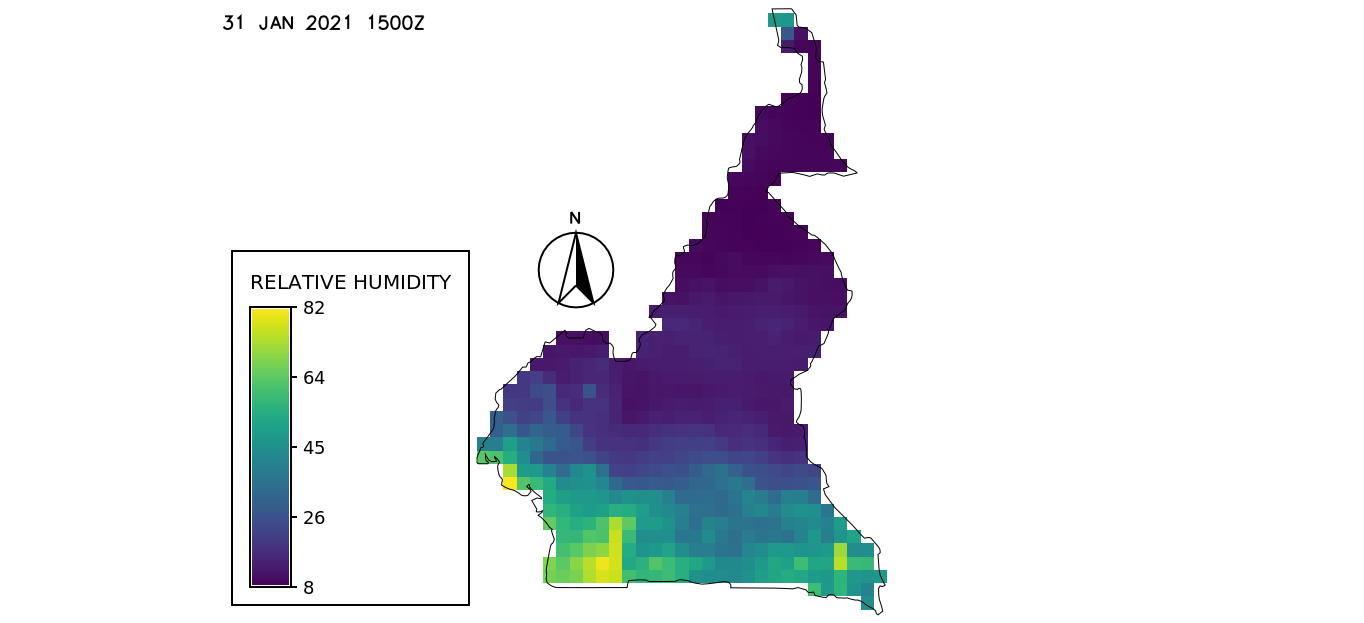
\includegraphics[scale=0.4]{rh15.png} %\cite{umhe}
\end{center}
\caption{Relative Humidity at 15:00 UTC}
\label{Relative Humidity at 15:00 UTC}%\cite{ABIA}
\end{figure}
\newpage
\subsection{Visualise Surface Pressure Chart}
\begin{figure}[H]
\begin{center}
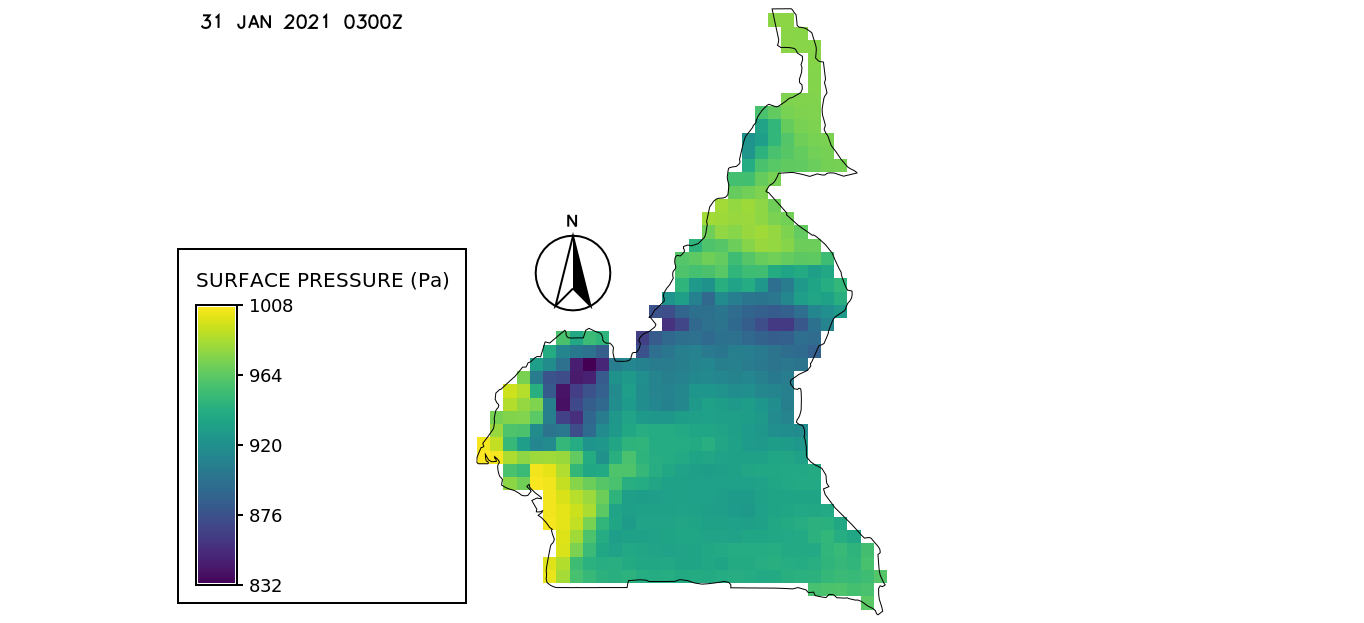
\includegraphics[scale=0.4]{sp03.png} %\cite{umhe}
\end{center}
\caption{Surface Pressure at 03:00 UTC}
\label{Surface Pressure  at 03:00 UTC}%\cite{ABIA}
\end{figure}

\begin{figure}[H]
\begin{center}
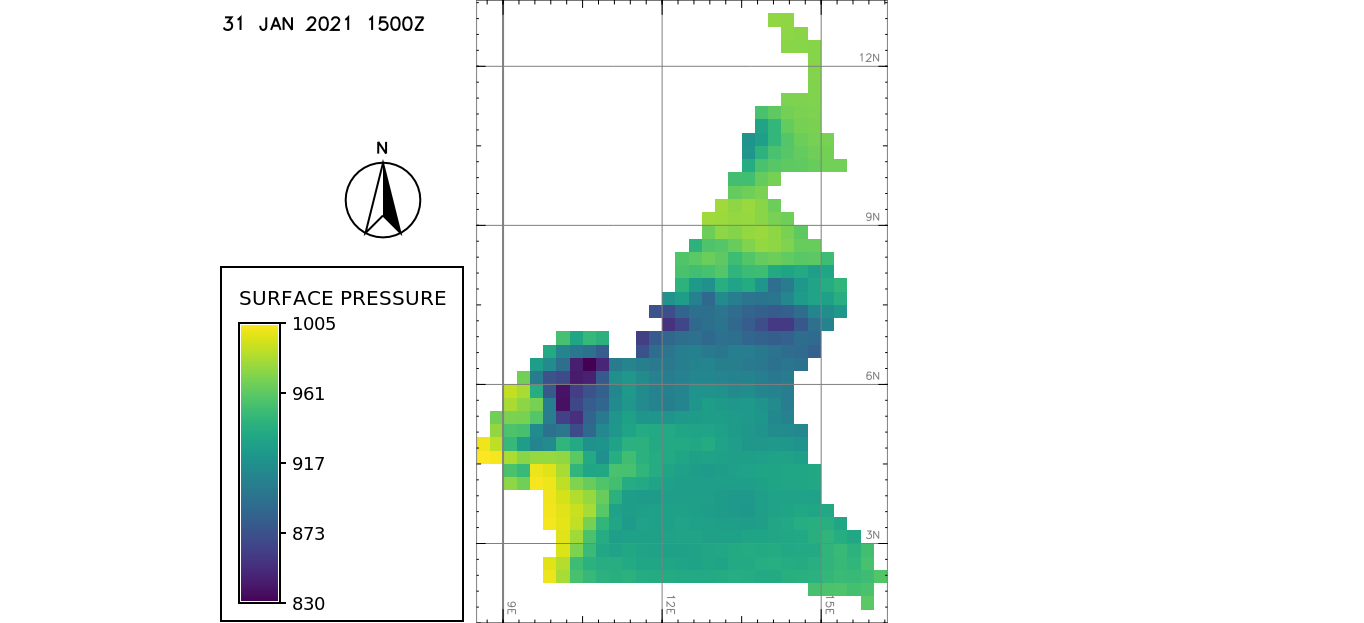
\includegraphics[scale=0.4]{sp15a.png} %\cite{umhe}
\end{center}
\caption{Surface Pressure  at 15:00 UTC}
\label{Surface Pressure  at 15:00 UTC}%\cite{ABIA}
\end{figure}
\newpage
\subsection{Visualise Wind Speed Chart}

\begin{figure}[H]
\begin{center}
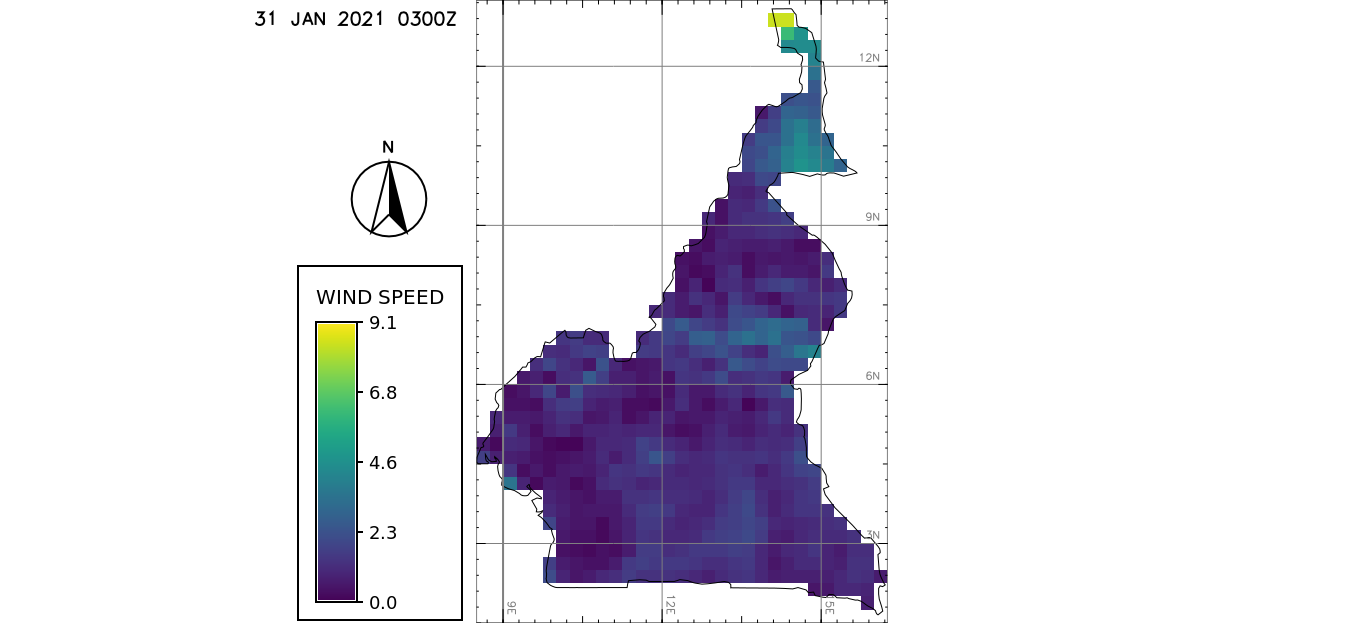
\includegraphics[scale=0.4]{ws03.png} %\cite{umhe}
\end{center}
\caption{Wind Speed at 03:00 UTC}
\label{Wind Speed at 03:00 UTC}%\cite{ABIA}
\end{figure}

\begin{figure}[H]
\begin{center}
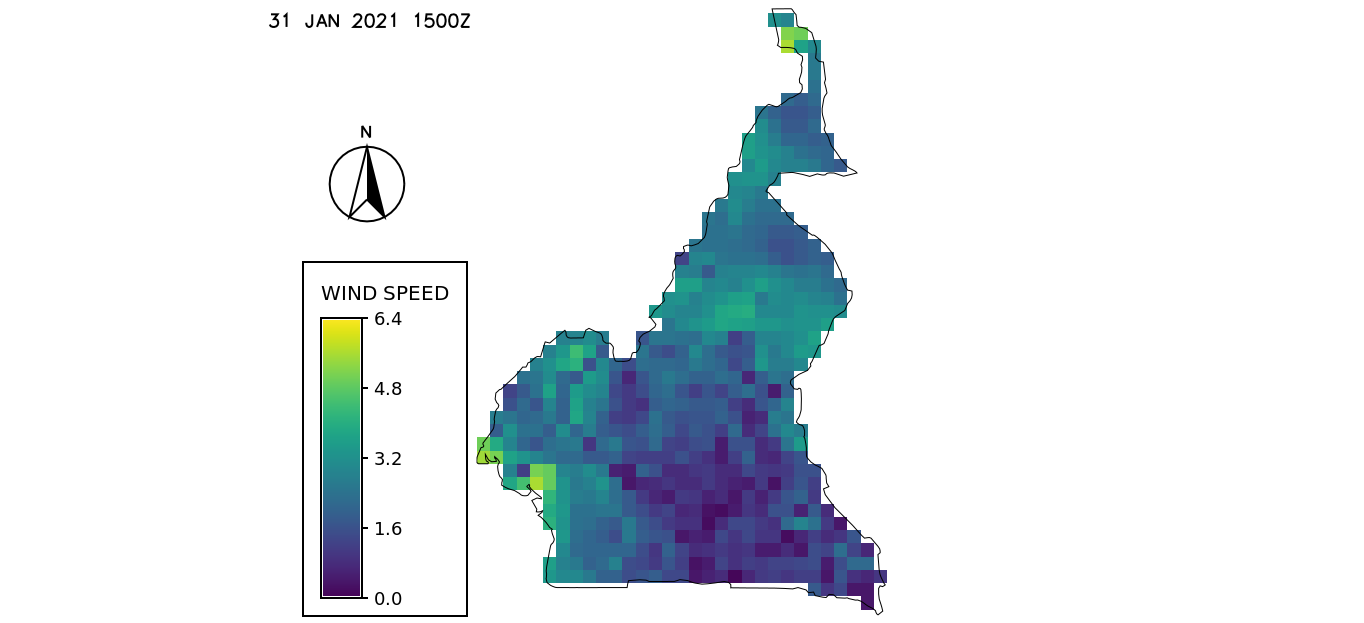
\includegraphics[scale=0.4]{ws15.png} %\cite{umhe}
\end{center}
\caption{Wind Speed at 15:00 UTC}
\label{Wind Speed at 15:00 UTC}%\cite{ABIA}
\end{figure}
\newpage
\section{Extract data}
\paragraph{}
Let us see how to extract raster values at particular observation points given as a vector layer. 
Here we will use aviation meteorological observation point in cameroon, to extract meterological parameters
Tair, Ws, P and Rh at observation time: 00:00,03:00,06:00,09:00,12:00,15:00,18:00 and 21:00.
\begin{lstlisting}[language=Bash]
#!/bin/bash
## This script process a single day GLDAS data and do all the required conversions needed for PySEBAL
## GENERAL ##
if [ -z "$GISBASE" ] ; then
    echo "You must be in GRASS GIS to run this program." >&2
    exit 1
fi
# Set a environment to enable overwrite by default
export GRASS_OVERWRITE=1
# Navigate to the folder containing single day .nc4 files
INDAT="/mnt/d/mi_is_project_data/2021/031" 
cd ${INDAT}
# set the computational region to Urmia Lake basin and set the computational resolution to 0.25 degrees
g.region vector=cmr res=0.25 -a
r.mask vect=cmr

# For loop to process all the .nc files in one go

for i in `ls GLDAS*.nc4`; do
    dt=`echo ${i}|cut -d. -f2-3`
    # Extract Air Temperature values 8 aviation meteorological station at time = dt and save the value in .csv file
    r.what -n map=GLDAS_NOAH025_3H_${dt}_Tair_final points=met_station  sep=comma output=a_temp_${dt}Z.csv
    # Extract Relative Humidity values 8 aviation meteorological station at time = dt and save the value in .csv file
    r.what -n map=GLDAS_NOAH025_3H_${dt}_Rh_final points=met_station  sep=comma output=a_rh_${dt}Z.csv
    # Extract Surface Pressure values 8 aviation meteorological station at time = dt and save the value in .csv file
    r.what -n map=GLDAS_NOAH025_3H_${dt}_Psurf_final points=met_station  sep=comma output=a_p_${dt}Z.csv
    # Extract Surface wind values 8 aviation meteorological station at time = dt and save the value in .csv file
    r.what -n map=GLDAS_NOAH025_3H_${dt}_Wind_final points=met_station  sep=comma output=a_ws_${dt}Z.csv
done
\end{lstlisting}
\paragraph{}
We save the script abive in the file \textcolor{magenta}{\scriptsize{extraction.sh}}, then run the bash script on Ubuntu using the command sh \textcolor{magenta}{\scriptsize{ sh extract.sh}}.
\newline
Let see how these file look in the directory
\begin{figure}[H]
\begin{center}
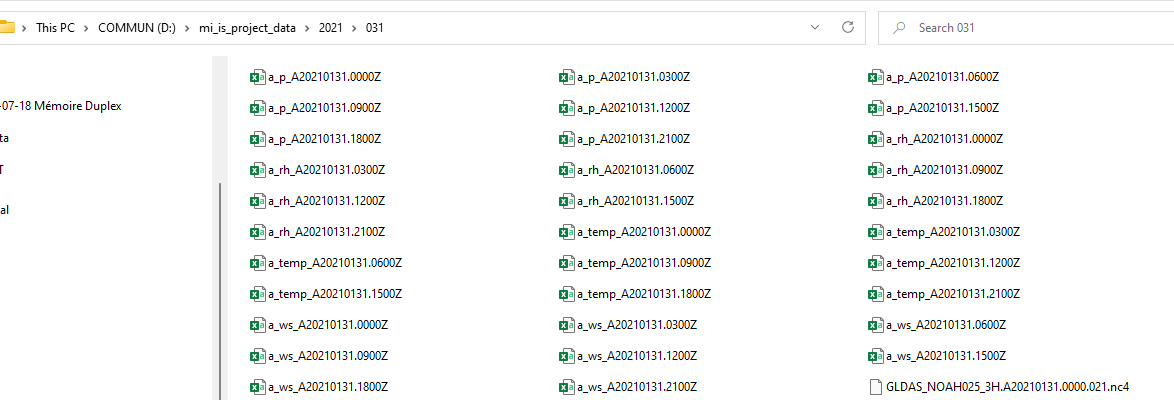
\includegraphics[scale=0.6]{csv2.png} %\cite{umhe}
\end{center}
\caption{File in directory}
\label{File in directory}%\cite{ABIA}
\end{figure}








\begin{table}[H]
\caption{Station Temperature extracted}
\label{Station Temperature extracted} 
\begin{center}
\begin{tabular}{|c|c|c|c|c|c|c|c|c|}
\hline
\multirow{2}*{ \small{\textbf{Time}}} & \multicolumn{8}{c|}{\small{\textbf{Temperature}}}\\
\cline{2-9}
  & \rotatebox {45}{\small{Yaounde}\,} & \rotatebox {45}{\small{Douala}\,}& \rotatebox {45}{\small{Garoua}\,} & \rotatebox {45}{\small{Maroua}\,} & \rotatebox {45}{\small{Ngaoundere}\,} & \rotatebox {45}{\small{Bafoussam}\,}& \rotatebox {45}{\small{Bertoua}\,} & \rotatebox {45}{\small{Bamenda}\,}\\ \hline
 \small{00:00}& \small{20.53 } & \small{NA }  & \small{22.69 } & \small{21.88 }     &\small{17.82 }   & \small{16.16 }     & \small{19.95}   &\small{ 16.23} \\[2pt] \hline
 \small{03:00} & \small{20.89} & \small{NA}  & \small{20.52} & \small{20.06}    & \small{17.20}  & \small{15.30 }   & \small{18.65}    & \small{15.74}   \\[2pt] \hline
 \small{06:00} & \small{20.56} & \small{NA } & \small{20.26} &\small{19.83}     & \small{17.15}  & \small{15.12 }   & \small{18.81}    & \small{15.93}   \\[2pt] \hline
 \small{09:00}  &  \small{28.19} & \small{NA }  & \small{29.55} &\small{27.78}  & \small{28.93 } & \small{28.41}    & \small{28.84}   & \small{29.24 }  \\[2pt] \hline
\small{12:00} & \small{32.79} & \small{NA } & \small{35.92} & \small{32.96}     &\small{32.38}   & \small{31.97}    & \small{37.50}    & \small{33.15 }  \\[2pt] \hline
\small{ 15:00} & \small{28.80} & \small{NA}  & \small{37.19} & \small{34.56}    &\small{31.21}   & \small{31.29}    & \small{34.05}    & \small{32.20}   \\[2pt] \hline
  \small{18:00}  & \small{24.12 }& \small{NA}  & \small{29.08} & \small{25.97}   & \small{22.35 } & \small{21.54}    & \small{25.18}    &\small{20.65}  \\[2pt] \hline
  \small{21:00} & \small{22.51 } & \small{NA}  & \small{25.92} & \small{24.92}   & \small{18.47}  & \small{18.26}    & \small{21.30}    & \small{17.94 } \\[2pt] \hline
 \end{tabular}
\end{center}
\end{table}









\begin{table}[H]
\caption{Station Relative Humidity extracted}
\label{Station Relative Humidity  extracted} 
\begin{center}
\begin{tabular}{|c|c|c|c|c|c|c|c|c|}
\hline
\multirow{2}*{ \small{\textbf{Time}}} & \multicolumn{8}{c|}{\small{\textbf{Relative Humidity}}}\\
\cline{2-9}
  & \rotatebox {45}{\small{Yaounde}\,} & \rotatebox {45}{\small{Douala}\,}& \rotatebox {45}{\small{Garoua}\,} & \rotatebox {45}{\small{Maroua}\,} & \rotatebox {45}{\small{Ngaoundere}\,} & \rotatebox {45}{\small{Bafoussam}\,}& \rotatebox {45}{\small{Bertoua}\,} & \rotatebox {45}{\small{Bamenda}\,}\\ \hline
\small{00:00}& \small{94.54} & \small{NA} & \small{16.14} & \small{20.95} & \small{21.98}  & \small{54.31}  & \small{58.72}  & \small{32.07}   \\[2pt] \hline
\small{03:00}& \small{90.14} & \small{NA} & \small{18.46} & \small{23.37} & \small{20.91}  & \small{40.82}  & \small{72.48}  & \small{29.25}   \\[2pt] \hline
\small{06:00}& \small{90.39} & \small{NA} & \small{19.23} & \small{23.40} & \small{23.16}  & \small{33.04}  & \small{91.95}  & \small{26.58}    \\[2pt] \hline
\small{09:00}& \small{54.54} & \small{NA} & \small{11.91} & \small{13.46} & \small{13.44}  & \small{14.43}  & \small{50.12}  & \small{13.34}   \\[2pt] \hline
\small{12:00}& \small{33.52} & \small{NA} & \small{8.54} & \small{9.56}   & \small{12.56}  & \small{14.23}  & \small{21.82}  & \small{12.27}   \\[2pt] \hline
\small{15:00}& \small{45.02}  & \small{NA} & \small{8.18} & \small{9.07}   & \small{13.46}  & \small{15.93}  & \small{23.29}  & \small{13.37}  \\[2pt] \hline
\small{18:00}& \small{60.96} & \small{NA} & \small{12.36} & \small{14.20} & \small{20.06}  & \small{32.72}  & \small{38.15}  & \small{28.70}   \\[2pt] \hline
\small{21:00}& \small{79.47} & \small{NA} & \small{14.99} & \small{14.70} & \small{25.07}  & \small{54.81}  & \small{54.48}  & \small{34.51}  \\[2pt] \hline
 \end{tabular}
\end{center}
\end{table}




                           
                            
                         
                            
                           
                          



\begin{table}[H]
\caption{Station Surface Pressure extracted}
\label{Station Surface Pressure  extracted} 
\begin{center}
\begin{tabular}{|c|c|c|c|c|c|c|c|c|}
\hline
\multirow{2}*{ \small{\textbf{Time}}} & \multicolumn{8}{c|}{\small{\textbf{Surface pressure}}}\\
\cline{2-9}
  & \rotatebox {45}{\small{Yaounde}\,} & \rotatebox {45}{\small{Douala}\,}& \rotatebox {45}{\small{Garoua}\,} & \rotatebox {45}{\small{Maroua}\,} & \rotatebox {45}{\small{Ngaoundere}\,} & \rotatebox {45}{\small{Bafoussam}\,}& \rotatebox {45}{\small{Bertoua}\,} & \rotatebox {45}{\small{Bamenda}\,}\\ \hline
\small{00:00}& \small{930.2783} & \small{NA} & \small{979.7773} & \small{962.4352} & \small{889.6512}  & \small{871.1833}  & \small{933.2983}  & \small{873.8692}   \\[2pt] \hline
\small{03:00}& \small{929.7397} & \small{NA} & \small{979.4847} & \small{961.8867} & \small{888.5327}  & \small{870.0627}  & \small{932.4217}  & \small{872.4927}   \\[2pt] \hline
\small{06:00}& \small{930.5676} & \small{NA} & \small{981.7227} & \small{963.8837} & \small{890.0356}  & \small{871.6027}  & \small{933.8506}  & \small{873.8066}    \\[2pt] \hline
\small{09:00}& \small{931.4058} & \small{NA} & \small{982.3198} & \small{964.6767} & \small{890.5017}  & \small{872.1998}  & \small{934.3908}  & \small{874.4767}   \\[2pt] \hline
\small{12:00}& \small{928.5176} & \small{NA} & \small{979.0986} & \small{962.0646} & \small{888.1417}  & \small{869.7606}  & \small{931.1577}  & \small{871.7536 }   \\[2pt] \hline
\small{15:00}& \small{925.8957} & \small{NA} & \small{975.8347} & \small{959.1037} & \small{886.0237}  & \small{867.2417}  & \small{928.1847 }  & \small{869.2897}  \\[2pt] \hline
\small{18:00}& \small{929.0854} & \small{NA} & \small{978.3014} & \small{961.4464} & \small{888.9214}  & \small{870.0524}  & \small{930.8405}  & \small{872.8555}   \\[2pt] \hline
\small{21:00}& \small{930.7338} & \small{NA} & \small{979.9328} & \small{962.7498} & \small{890.4208}  & \small{871.8887}  & \small{932.9238}  & \small{874.6868}  \\[2pt] \hline
 \end{tabular}
\end{center}
\end{table}






\section{Comparison between value extracted and those obseved at met station}
\paragraph{}

 
\begin{table}[H]
\caption{Satellite and station data at Garoua station}
\label{Station Wind Speed extracted} 
\begin{center}
\begin{tabular}{|c|c|c|c|c|c|c|}
\hline
\multirow{2}*{ \small{\textbf{Time}}} & \multicolumn{6}{c|}{\small{\textbf{Garoua meteorological station}}}\\
\cline{2-7}
  & \rotatebox {45}{\small{Tair_satellite}\,} & \rotatebox {45}{\small{Tair_station}\,}& \rotatebox {45}{\small{Rh_satellite}\,} & \rotatebox {45}{\small{Rh_station}\,} & \rotatebox {45}{\small{P_satellite}\,} & \rotatebox {45}{\small{P_station}\,}\\ \hline
\small{00:00}& \small{22.69231567} & \small{24}   & \small{16.14377} & \small{31} & \small{979.7773}  & \small{982.6}    \\[2pt] \hline
\small{03:00}& \small{20.52959595} & \small{20.2} & \small{18.45571} & \small{39} & \small{979.4847}  & \small{982.5}    \\[2pt] \hline
\small{06:00}& \small{20.26201782} & \small{19.5} & \small{19.2371}  & \small{43} & \small{981.7227}  & \small{983.9}     \\[2pt] \hline
\small{09:00}& \small{29.55059204} & \small{29}   & \small{11.90664} & \small{25} & \small{982.3198}  & \small{984.9}    \\[2pt] \hline
\small{12:00}& \small{35.92055664} & \small{34}   & \small{8.537706} & \small{15} & \small{979.0986}  & \small{981.8}   \\[2pt] \hline
\small{15:00}& \small{37.19307861} & \small{36}   & \small{8.181383} & \small{17} & \small{975.8347}  & \small{979.3}   \\[2pt] \hline
\small{18:00}& \small{29.08526001} & \small{30.5} & \small{12.35657} & \small{27} & \small{978.3014}  & \small{980.4}     \\[2pt] \hline
\small{21:00}& \small{25.92067871} & \small{25.9} & \small{14.98635} & \small{31} & \small{979.9328}  & \small{982.5}    \\[2pt] \hline
 \end{tabular}
\end{center}
\end{table}

               
               
               
               
               
               
               
               




\begin{table}[H]
\caption{Station Wind Speed extracted}
\label{Station Wind Speed extracted} 
\begin{center}
\begin{tabular}{|c|c|c|c|c|c|c|c|c|}
\hline
\multirow{2}*{ \small{\textbf{Time}}} & \multicolumn{8}{c|}{\small{\textbf{Wind Speed}}}\\
\cline{2-9}
  & \rotatebox {45}{\small{Yaounde}\,} & \rotatebox {45}{\small{Douala}\,}& \rotatebox {45}{\small{Garoua}\,} & \rotatebox {45}{\small{Maroua}\,} & \rotatebox {45}{\small{Ngaoundere}\,} & \rotatebox {45}{\small{Bafoussam}\,}& \rotatebox {45}{\small{Bertoua}\,} & \rotatebox {45}{\small{Bamenda}\,}\\ \hline
\small{00:00}& \small{E} & \small{F} & \small{M} & \small{E} & \small{F}  & \small{E}  & \small{E}  & \small{E}   \\[2pt] \hline
\small{03:00}& \small{M} & \small{M} & \small{M} & \small{E} & \small{M}  & \small{M}  & \small{M}  & \small{E}   \\[2pt] \hline
\small{06:00}& \small{E} & \small{E} & \small{E} & \small{E} & \small{E}  & \small{E}  & \small{E}  & \small{E}    \\[2pt] \hline
\small{09:00}& \small{E} & \small{E} & \small{E} & \small{M} & \small{E}  & \small{F}  & \small{F}  & \small{E}   \\[2pt] \hline
\small{12:00}& \small{E} & \small{E} & \small{M} & \small{F} & \small{E}  & \small{F}  & \small{F}  & \small{E}   \\[2pt] \hline
\small{15:00}& \small{F} & \small{F} & \small{F} & \small{M} & \small{F}  & \small{M}  & \small{M}  & \small{E}  \\[2pt] \hline
\small{18:00}& \small{M} & \small{F} & \small{F} & \small{M} & \small{F}  & \small{E}  & \small{E}  & \small{E}   \\[2pt] \hline
\small{21:00}& \small{F} & \small{F} & \small{F} & \small{E} & \small{F}  & \small{E}  & \small{E}  & \small{E}  \\[2pt] \hline
 \end{tabular}
\end{center}
\end{table}





\section{Share results with scientific commmunity}
\paragraph{}